

\chapter{Pruebas}

Una vez terminada la aplicación web por completo, en este apartado se recoge la batería de pruebas realizadas para comprobar el rendimiento y sobretodo, la eficacia de la aplicación a la hora de operar en la vida real.	\newline

\section{Diseño del banco de pruebas}

En esta sección se expone el diseño del banco de pruebas.\newline

Para las pruebas se utilizará la funcionalidad de backtesting con estrategia; y se usará el método implementado de Wyckoff.\newline

El año en el que se simulará la operativa será 2018. Elijo este año para tener la mínima repercusión posible en los resultados del backtesting debido a la pandemia del \textit{COVID-19}. Comenzaremos también a partir del mes de \textit{febrero} para evitar días sin operar por culpa del fin de las fiestas de Navidad que transcurre en \textit{enero}. \newline

Detallo a continuación los mercados financieros que vamos a operar:\newline

\begin{itemize}
	\item \textbf{Euro vs US Dollar}: precio de cambio de Euro a Dólar estadounidense. Es una de las divisas más famosas en el trading de divisas o \textit{Forex}.
	\item \textbf{XAU vs US Dollar}: precio del oro en dólares estadounidenses. Metal precioso disponible en \textit{MetaTrader5}.
	\item \textbf{XAG vs Euro}: precio de la plata en euros. Metal precioso disponible en \textit{MetaTrader5}.
	\item \textbf{XBR vs US Dollar}: precio de cambio del petróleo \textit{Brent} a dólares estadounidenses. Materia prima o energía disponible en \textit{MetaTrader5}.
	\item \textbf{XNG vs US Dollar}: precio de cambio del gas natural a dólares estadounidenses. Materia prima o energía disponible en \textit{MetaTrader5}.
\end{itemize}

Una vez listamos los mercados a operar, menciono la temporalidad que vamos a usar para cada uno y el tiempo que pretendemos estar operando en dicho mercado con nuestro algoritmo. Antes de destacar en la lista, cabe comentar los tipos de trading en cuanto a tiempo se refiere:\newline

\begin{itemize}
	\item \textbf{Scalping}: operar a muy corto plazo abriendo y cerrando posiciones en pocos minutos o segundos. No vamos a simular este comportamiento debido a que no tenemos capacidad de operar en tan poco tiempo.
	\item \textbf{Day Trading}: operar a corto plazo en el mismo día del inicio de la operación. En este caso podemos simular la operativa con los marcos de \textit{Min15} y \textit{H1}.
	\item \textbf{Swing Trading}: consiste en una operativa a medio plazo en el que las operaciones se cierran en días. Podemos usar las temporalidades de \textit{H4} o \textit{D1}.
	\item \textbf{Largo plazo}: perfiles de inversión a largo plazo. Consiste en mantener abiertas posiciones durante semanas o meses. No simulamos este comportamiento por la falta de temporalidades más altas.
\end{itemize}

Finalmente, comento las temporalidades usadas para cada mercado y durante cuánto tiempo probaremos cada una:\newline

\begin{itemize}
	\item \textit{Min15}: 8 horas y 3 días.
	\item \textit{H1}: 3 días y 5 días.
	\item \textit{H4}: 5 días y 14 días.
	\item \textit{D1}: 1 mes y 3 meses.
\end{itemize}

Una vez detallado el banco de pruebas a seguir, resumo haciendo un recuento del total de operativas a realizar:\newline

\textit{5 mercados x 4 temporalidades x 2 periodos distintos = 40 ejecuciones de backtesting} \newline

\section{Pruebas del método de Wyckoff en backtesting}

Siguiendo el diseño propuesto en el punto anterior, realizo cada una de las pruebas a partir de febrero de 2018, usando la funcionalidad de \textit{backtesting} que simula una operativa en tiempo real.\newline

En el caso de los materiales preciosos (oro y plata), se ha aumentado el período de trading, debido a que por cómo es su comportamiento, el algoritmo tarda más en elegir posibles compras o ventas. Se ha hecho lo mismo para las materias primas (brent y gas natural)\newline

Debido a la gran cantidad de gráficos resultado, representaré la primera con todo el \textit{verbose}: gráficos decisiones, etc; y dejaré las siguientes con solo las operaciones y el balance final.\newline

Como se puede apreciar, en las gráficas vemos las franjas azules que representan la detección de tendencias para luego entrar a operar. Podemos también ver las decisiones tomadas por el algoritmo para incluir cada una de las operaciones.

\subsection{EURUSD}

\subsubsection{Temporalidad: \textit{Min15}}

\paragraph{8 horas} 

ACCIONES REALIZADAS:\\

No se ha realizado ninguna operación en el tiempo transcurrido.

\paragraph{3 días}

ACCIONES REALIZADAS:\\

- Orden número 1: COMPRA. Realizada con fecha y hora: 05/02 20:30. Valor compra = 1.24207. SL = 1.240084. TP = 1.246042. RESULTADO: FALLIDA. PÉRDIDAS OBTENIDAS: -0.0019860000000000433.\\

Decisiones tomadas por el algoritmo: - Objetivo potencial bajista cumplido, indicadores cumplidos = 1. En la gráfica se observa de color azul la franja en la que se ha detectado la tendencia - Minimo mas alto, indicadores cumplidos = 2 - Minimo mas alto, indicadores cumplidos = 3 - Tendencia bajista se ha roto, indicadores cumplidos = 4 - Minimo mas alto, indicadores cumplidos = 5 DECISION: Decido comprar tras superar los tests de Wyckoff \newline

- Orden número 2: VENTA. Realizada con fecha y hora: 07/02 00:00. Valor venta = 1.23742. SL = 1.240632. TP = 1.230996. RESULTADO: ACIERTO. BENEFICIOS OBTENIDOS: 0.006423999999999985.\\

Decisiones tomadas por el algoritmo: - Objetivo potencial alcista cumplido, indicadores cumplidos = 1. En la gráfica se observa de color azul la franja en la que se ha detectado la tendencia - Tendencia alcista se ha roto, indicadores cumplidos = 2 - Minimo mas bajo, indicadores cumplidos = 3 - Maximo mas bajo, indicadores cumplidos = 4 - Maximo mas bajo, indicadores cumplidos = 5 DECISION: Decido vender tras superar los tests de Wyckoff\newline

- Orden número 3: COMPRA. Realizada con fecha y hora: 08/02 01:45. Valor compra = 1.22703. SL = 1.22408. TP = 1.23293. RESULTADO: FALLIDA. PÉRDIDAS OBTENIDAS: -0.002950000000000008.\\

Decisiones tomadas por el algoritmo: - Objetivo potencial bajista cumplido, indicadores cumplidos = 1. En la gráfica se observa de color azul la franja en la que se ha detectado la tendencia - Tendencia bajista se ha roto, indicadores cumplidos = 2 - Minimo mas alto, indicadores cumplidos = 3 - Minimo mas alto, indicadores cumplidos = 4 - Minimo mas alto, indicadores cumplidos = 5 DECISION: Decido comprar tras superar los tests de Wyckoff\newline

\color{blue}
BALANCE OBTENIDO:\newline

0.0014879999999999338\newline
\color{black}

\begin{figure}[h]
	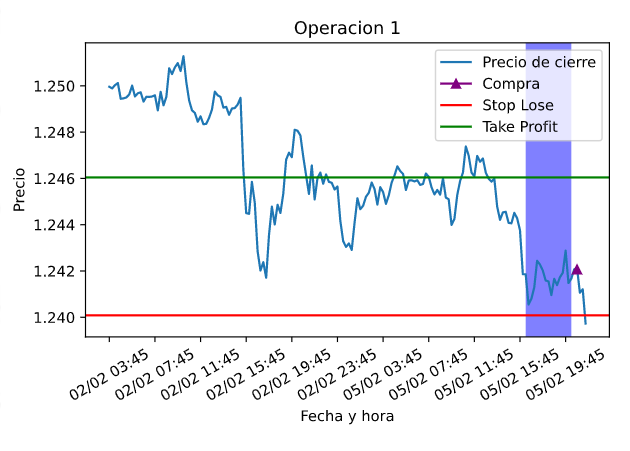
\includegraphics[width=1\textwidth]{imagenes/pruebas/EURUSD/min15_3dias.png}	
	\caption{EURUSD, Min15 durante 3 días, operacion 1.}
\end{figure}

\begin{figure}[h]
	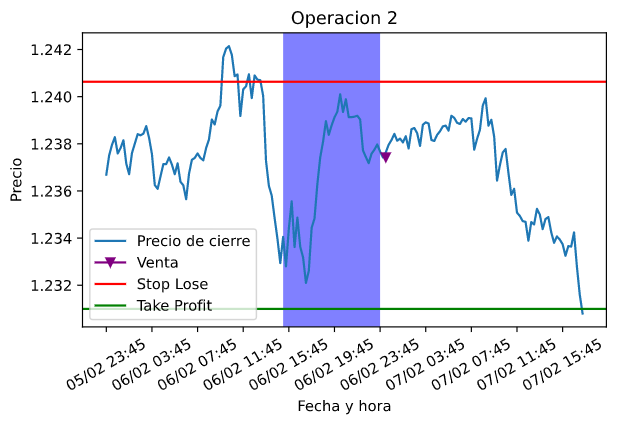
\includegraphics[width=1\textwidth]{imagenes/pruebas/EURUSD/min15_3dias_2.png}	
	\caption{EURUSD, Min15 durante 3 días, operacion 2.}
\end{figure}

\begin{figure}[h]
	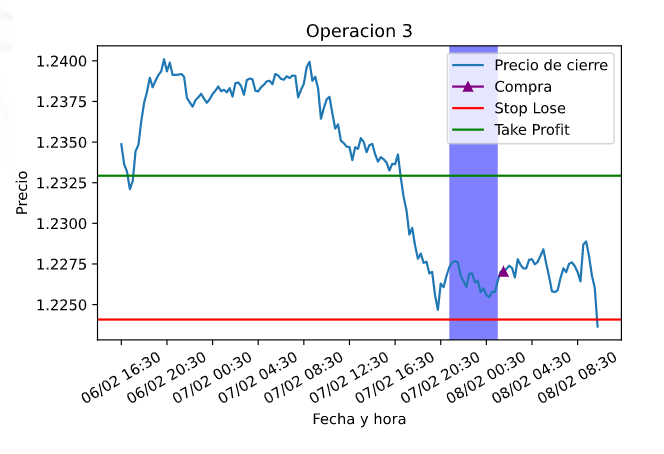
\includegraphics[width=1\textwidth]{imagenes/pruebas/EURUSD/min15_3dias_3.png}	
	\caption{EURUSD, Min15 durante 3 días, operacion 3.}
\end{figure}


\subsubsection{Temporalidad: \textit{H1}}

\paragraph{3 días}

ACCIONES REALIZADAS:\\

- Orden número 1: VENTA. Realizada con fecha y hora: 07/02 09:00. Valor venta = 1.2383. SL = 1.240432. TP = 1.234036. RESULTADO: ACIERTO. BENEFICIOS OBTENIDOS: 0.0042640000000000455.\newline

\color{blue}
BALANCE OBTENIDO:\newline

0.0042640000000000455\newline
\color{black}
\paragraph{5 días}

ACCIONES REALIZADAS:\\

- Orden número 1: COMPRA. Realizada con fecha y hora: 14/02 03:00. Valor compra = 1.23548. SL = 1.2345979999999999. TP = 1.237244. RESULTADO: ACIERTO. BENEFICIOS OBTENIDOS: 0.0017640000000000988.\newline

- Orden número 2: VENTA. Realizada con fecha y hora: 15/02 16:00. Valor venta = 1.24985. SL = 1.25061. TP = 1.2483299999999997. RESULTADO: ACIERTO. BENEFICIOS OBTENIDOS: 0.0015200000000001879.\newline

\color{blue}
BALANCE OBTENIDO:\newline

0.0032840000000002867\newline
\color{black}
\subsubsection{Temporalidad: \textit{H4}}

\paragraph{14 días}

ACCIONES REALIZADAS:\\

No se ha realizado ninguna operación en el tiempo transcurrido.

\paragraph{1 mes}

ACCIONES REALIZADAS:\\

- Orden número 1: VENTA. Realizada con fecha y hora: 12/02 16:00. Valor venta = 1.22754. SL = 1.22892. TP = 1.2247800000000002. RESULTADO: FALLIDA. PÉRDIDAS OBTENIDAS: -0.0013799999999999368.\newline

\color{blue}
BALANCE OBTENIDO:\newline

-0.0013799999999999368\newline
\color{black}

\subsubsection{Temporalidad: \textit{D1}}

\paragraph{1 mes}

ACCIONES REALIZADAS:\\

No se ha realizado ninguna operación en el tiempo transcurrido.

\paragraph{3 meses}

ACCIONES REALIZADAS:\\

- Orden número 1: COMPRA. Realizada con fecha y hora: 14/06 00:00. Valor compra = 1.15661. SL = 1.148564. TP = 1.172702. RESULTADO: ACIERTO. BENEFICIOS OBTENIDOS: 0.016091999999999995.\newline

\color{blue}
BALANCE OBTENIDO:\newline

0.016091999999999995\newline
\color{black}





\subsection{XAUUSD}

\subsubsection{Temporalidad: \textit{Min15}}

\paragraph{8 horas}

ACCIONES REALIZADAS:\\

No se ha realizado ninguna operación en el tiempo transcurrido

\paragraph{3 días}

ACCIONES REALIZADAS:\\

No se ha realizado ninguna operación en el tiempo transcurrido

\subsubsection{Temporalidad: \textit{H1}}

\paragraph{3 días}

ACCIONES REALIZADAS:\\

No se ha realizado ninguna operación en el tiempo transcurrido

\paragraph{5 días}

ACCIONES REALIZADAS:\\

No se ha realizado ninguna operación en el tiempo transcurrido

\subsubsection{Temporalidad: \textit{H4}}

\paragraph{5 días}

ACCIONES REALIZADAS:\\

No se ha realizado ninguna operación en el tiempo transcurrido

\paragraph{2 meses}

ACCIONES REALIZADAS:\\

- Orden número 1: VENTA. Realizada con fecha y hora: 26/02 16:00. Valor venta = 1325.82. SL = 1349.7359999999999. TP = 1277.988. RESULTADO: ACIERTO. BENEFICIOS OBTENIDOS: 47.83199999999988.\newline


\color{blue}
BALANCE OBTENIDO:\newline

47.83199999999988\newline
\color{black}

\subsubsection{Temporalidad: \textit{D1}}

\paragraph{3 meses}

ACCIONES REALIZADAS:\\

No se ha realizado ninguna operación en el tiempo transcurrido

\paragraph{12 meses}

ACCIONES REALIZADAS:\\

No se ha realizado ninguna operación en el tiempo transcurrido






\subsection{XAGEUR}

\subsubsection{Temporalidad: \textit{Min15}}

\paragraph{8 horas}

ACCIONES REALIZADAS:\\

No se ha realizado ninguna operación en el tiempo transcurrido

\paragraph{3 días}

ACCIONES REALIZADAS:\\

No se ha realizado ninguna operación en el tiempo transcurrido

\subsubsection{Temporalidad: \textit{H1}}

\paragraph{3 días}

ACCIONES REALIZADAS:\\

No se ha realizado ninguna operación en el tiempo transcurrido

\paragraph{5 días}

ACCIONES REALIZADAS:\\

No se ha realizado ninguna operación en el tiempo transcurrido

\subsubsection{Temporalidad: \textit{H4}}

\paragraph{5 días}

ACCIONES REALIZADAS:\\

No se ha realizado ninguna operación en el tiempo transcurrido

\paragraph{2 meses}

ACCIONES REALIZADAS:\\

- Orden número 1: COMPRA. Realizada con fecha y hora: 07/03 00:00. Valor compra = 13.367. SL = 13.2934. TP = 13.514200000000002. RESULTADO: ACIERTO. BENEFICIOS OBTENIDOS: 0.14720000000000155.\newline

- Orden número 2: VENTA. Realizada con fecha y hora: 19/03 16:00. Valor venta = 13.545. SL = 13.6006. TP = 13.4338. RESULTADO: FALLIDA. PÉRDIDAS OBTENIDAS: -0.055600000000000094.\newline

- Orden número 3: VENTA. Realizada con fecha y hora: 02/04 04:00. Valor venta = 13.446. SL = 13.5322. TP = 13.2736. RESULTADO: FALLIDA. PÉRDIDAS OBTENIDAS: -0.08619999999999983.\newline

\color{blue}
BALANCE OBTENIDO:\newline

0.005400000000001626\newline
\color{black}

\subsubsection{Temporalidad: \textit{D1}}

\paragraph{3 meses}

ACCIONES REALIZADAS:\\

No se ha realizado ninguna operación en el tiempo transcurrido

\paragraph{12 meses}

ACCIONES REALIZADAS:\\

No se ha realizado ninguna operación en el tiempo transcurrido





\subsection{XBRUSD}

\subsubsection{Temporalidad: \textit{Min15}}

\paragraph{8 horas}

ACCIONES REALIZADAS:\\

No se ha realizado ninguna operación en el tiempo transcurrido

\paragraph{3 días}

ACCIONES REALIZADAS:\\

No se ha realizado ninguna operación en el tiempo transcurrido

\subsubsection{Temporalidad: \textit{H1}}

\paragraph{3 días}

ACCIONES REALIZADAS:\\

No se ha realizado ninguna operación en el tiempo transcurrido

\paragraph{5 días}

ACCIONES REALIZADAS:\\

No se ha realizado ninguna operación en el tiempo transcurrido

\subsubsection{Temporalidad: \textit{H4}}

\paragraph{5 días}

ACCIONES REALIZADAS:\\

No se ha realizado ninguna operación en el tiempo transcurrido

\paragraph{2 meses}

ACCIONES REALIZADAS:\\

- Orden número 1: VENTA. Realizada con fecha y hora: 20/02 12:00. Valor venta = 65.78. SL = 66.66. TP = 64.02000000000001. RESULTADO: FALLIDA. PÉRDIDAS OBTENIDAS: -0.8799999999999955.\newline

- Orden número 2: VENTA. Realizada con fecha y hora: 01/03 16:00. Valor venta = 64.73. SL = 66.7. TP = 60.790000000000006. RESULTADO: FALLIDA. PÉRDIDAS OBTENIDAS: -1.9699999999999989.\newline


\color{blue}
BALANCE OBTENIDO:\newline

-2.8499999999999943\newline
\color{black}

\subsubsection{Temporalidad: \textit{D1}}

\paragraph{3 meses}

ACCIONES REALIZADAS:\\

No se ha realizado ninguna operación en el tiempo transcurrido

\paragraph{12 meses}

ACCIONES REALIZADAS:\\

No se ha realizado ninguna operación en el tiempo transcurrido




\subsection{XNGUSD}

\subsubsection{Temporalidad: \textit{Min15}}

\paragraph{8 horas}

ACCIONES REALIZADAS:\\

No se ha realizado ninguna operación en el tiempo transcurrido

\paragraph{3 días}

ACCIONES REALIZADAS:\\

No se ha realizado ninguna operación en el tiempo transcurrido

\subsubsection{Temporalidad: \textit{H1}}

\paragraph{3 días}

ACCIONES REALIZADAS:\\

No se ha realizado ninguna operación en el tiempo transcurrido

\paragraph{5 días}

ACCIONES REALIZADAS:\\

No se ha realizado ninguna operación en el tiempo transcurrido

\subsubsection{Temporalidad: \textit{H4}}

\paragraph{5 días}

ACCIONES REALIZADAS:\\

No se ha realizado ninguna operación en el tiempo transcurrido

\paragraph{2 meses}

ACCIONES REALIZADAS:\\

- Orden número 1: COMPRA. Realizada con fecha y hora: 27/06 12:00. Valor compra = 2.293. SL = 2.133. TP = 2.6130000000000004. RESULTADO: FALLIDA. PÉRDIDAS OBTENIDAS: -0.16000000000000014.\newline

- Orden número 2: COMPRA. Realizada con fecha y hora: 31/07 16:00. Valor compra = 2.262. SL = 2.128. TP = 2.53. RESULTADO: FALLIDA. PÉRDIDAS OBTENIDAS: -0.1339999999999999.\newline


\color{blue}
BALANCE OBTENIDO:\newline

-0.29400000000000004\newline
\color{black}

\subsubsection{Temporalidad: \textit{D1}}

\paragraph{3 meses}

ACCIONES REALIZADAS:\\

No se ha realizado ninguna operación en el tiempo transcurrido

\paragraph{12 meses}

ACCIONES REALIZADAS:\\

- Orden número 1: VENTA. Realizada con fecha y hora: 26/12 00:00. Valor venta = 2.276. SL = 2.4206000000000003. TP = 1.9867999999999988. RESULTADO: ACIERTO. BENEFICIOS OBTENIDOS: 0.289200000000001.\newline


\color{blue}
BALANCE OBTENIDO:\newline

0.289200000000001\newline
\color{black}


\paragraph{Prueba final: EURUSD}

Debido al éxito en los resultados de EURUSD, he lanzado un test en backtesting sólo para este mercado. La temporalidad usada ha sido de H1 y se simula un uso del algoritmo durante 4 años.\newline

Durante estos 4 años: desde 2017 hasta 2021, hemos ordenado un total de 255 operaciones de compra venta y hemos obtenido unos beneficios de: 0.09591399999999672 \newline

A pesar de que no es gran cantidad, es un entero positivo, lo que indica que en todo ese tiempo hemos estado con balance positivo. Si usamos de manera adecuada los lotes, podríamos haber obtenido una mayor cantidad de dinero. El uso de lotes o lotaje se explica en las conclusiones.\newline

